\section*{Author biographies}

\setlength\intextsep{0pt} % to bring image and text on same level
\begin{wrapfigure}{l}{25mm} 
    \includegraphics[width=1in,height=1.25in,clip,keepaspectratio]{illustrations/photo_sascha.png}
\end{wrapfigure}\par
\noindent \textbf{Sascha Kirch} is a doctoral student at UNED, Spain. His research focuses on self-supervised multi-modal generative deeplearning. He received his M.Sc. degree in Electronic Systems for Communication and Information from UNED, Spain. He received his B.Eng. degree in electrical engineering from the Cooperative State University Baden-Wuerttemberg (DHBW), Germany. Sascha is member of IEEE’s honor society Eta Kappa Nu as part of the chapter Nu Alpha.\\

\setlength\intextsep{0pt} % to bring image and text on same level
\begin{wrapfigure}{l}{25mm} 
    
\includegraphics[width=1in,height=1.25in,clip,keepaspectratio]{illustrations/photo_val.jpg}
\end{wrapfigure}\par
\noindent \textbf{Valeria Olyunina} is a 3D Computer Vision Engineer at Volograms Ltd. Her work is centered around volumetric reconstruction of people from video, including research into AI-generated shape estimation and other AI applicable to the subject. She received her M.Sc. degree in Computer Science specialising in Augmented Reality from Trinity College Dublin, Ireland. She also has Postgraduate Diploma in Mathematical modelling and Numerical Solutions from University College Cork, Ireland.\\

\setlength\intextsep{0pt} % to bring image and text on same level
\begin{wrapfigure}{l}{25mm} 
    
\includegraphics[width=1in,height=1.25in,clip,keepaspectratio]{illustrations/photo_jan.jpg}
\end{wrapfigure}\par
\noindent \textbf{Jan Ondřej} is Co-Founder and CTO of Volograms, where he has been since 2018. Previously, he was a postdoctoral researcher at Trinity College Dublin and Disney Research Los Angeles. He obtained M.Sc. in Computer Science in 2007 from Czech Technical University in Prague and his Ph.D. in 2011 from INRIA Rennes, in France. Since 2008 he worked as a researcher in several national and European projects related to volumetric video, animation of virtual humans and crowds, and application of VR/AR technologies.\\

\setlength\intextsep{0pt} % to bring image and text on same level
\begin{wrapfigure}{l}{25mm} 
    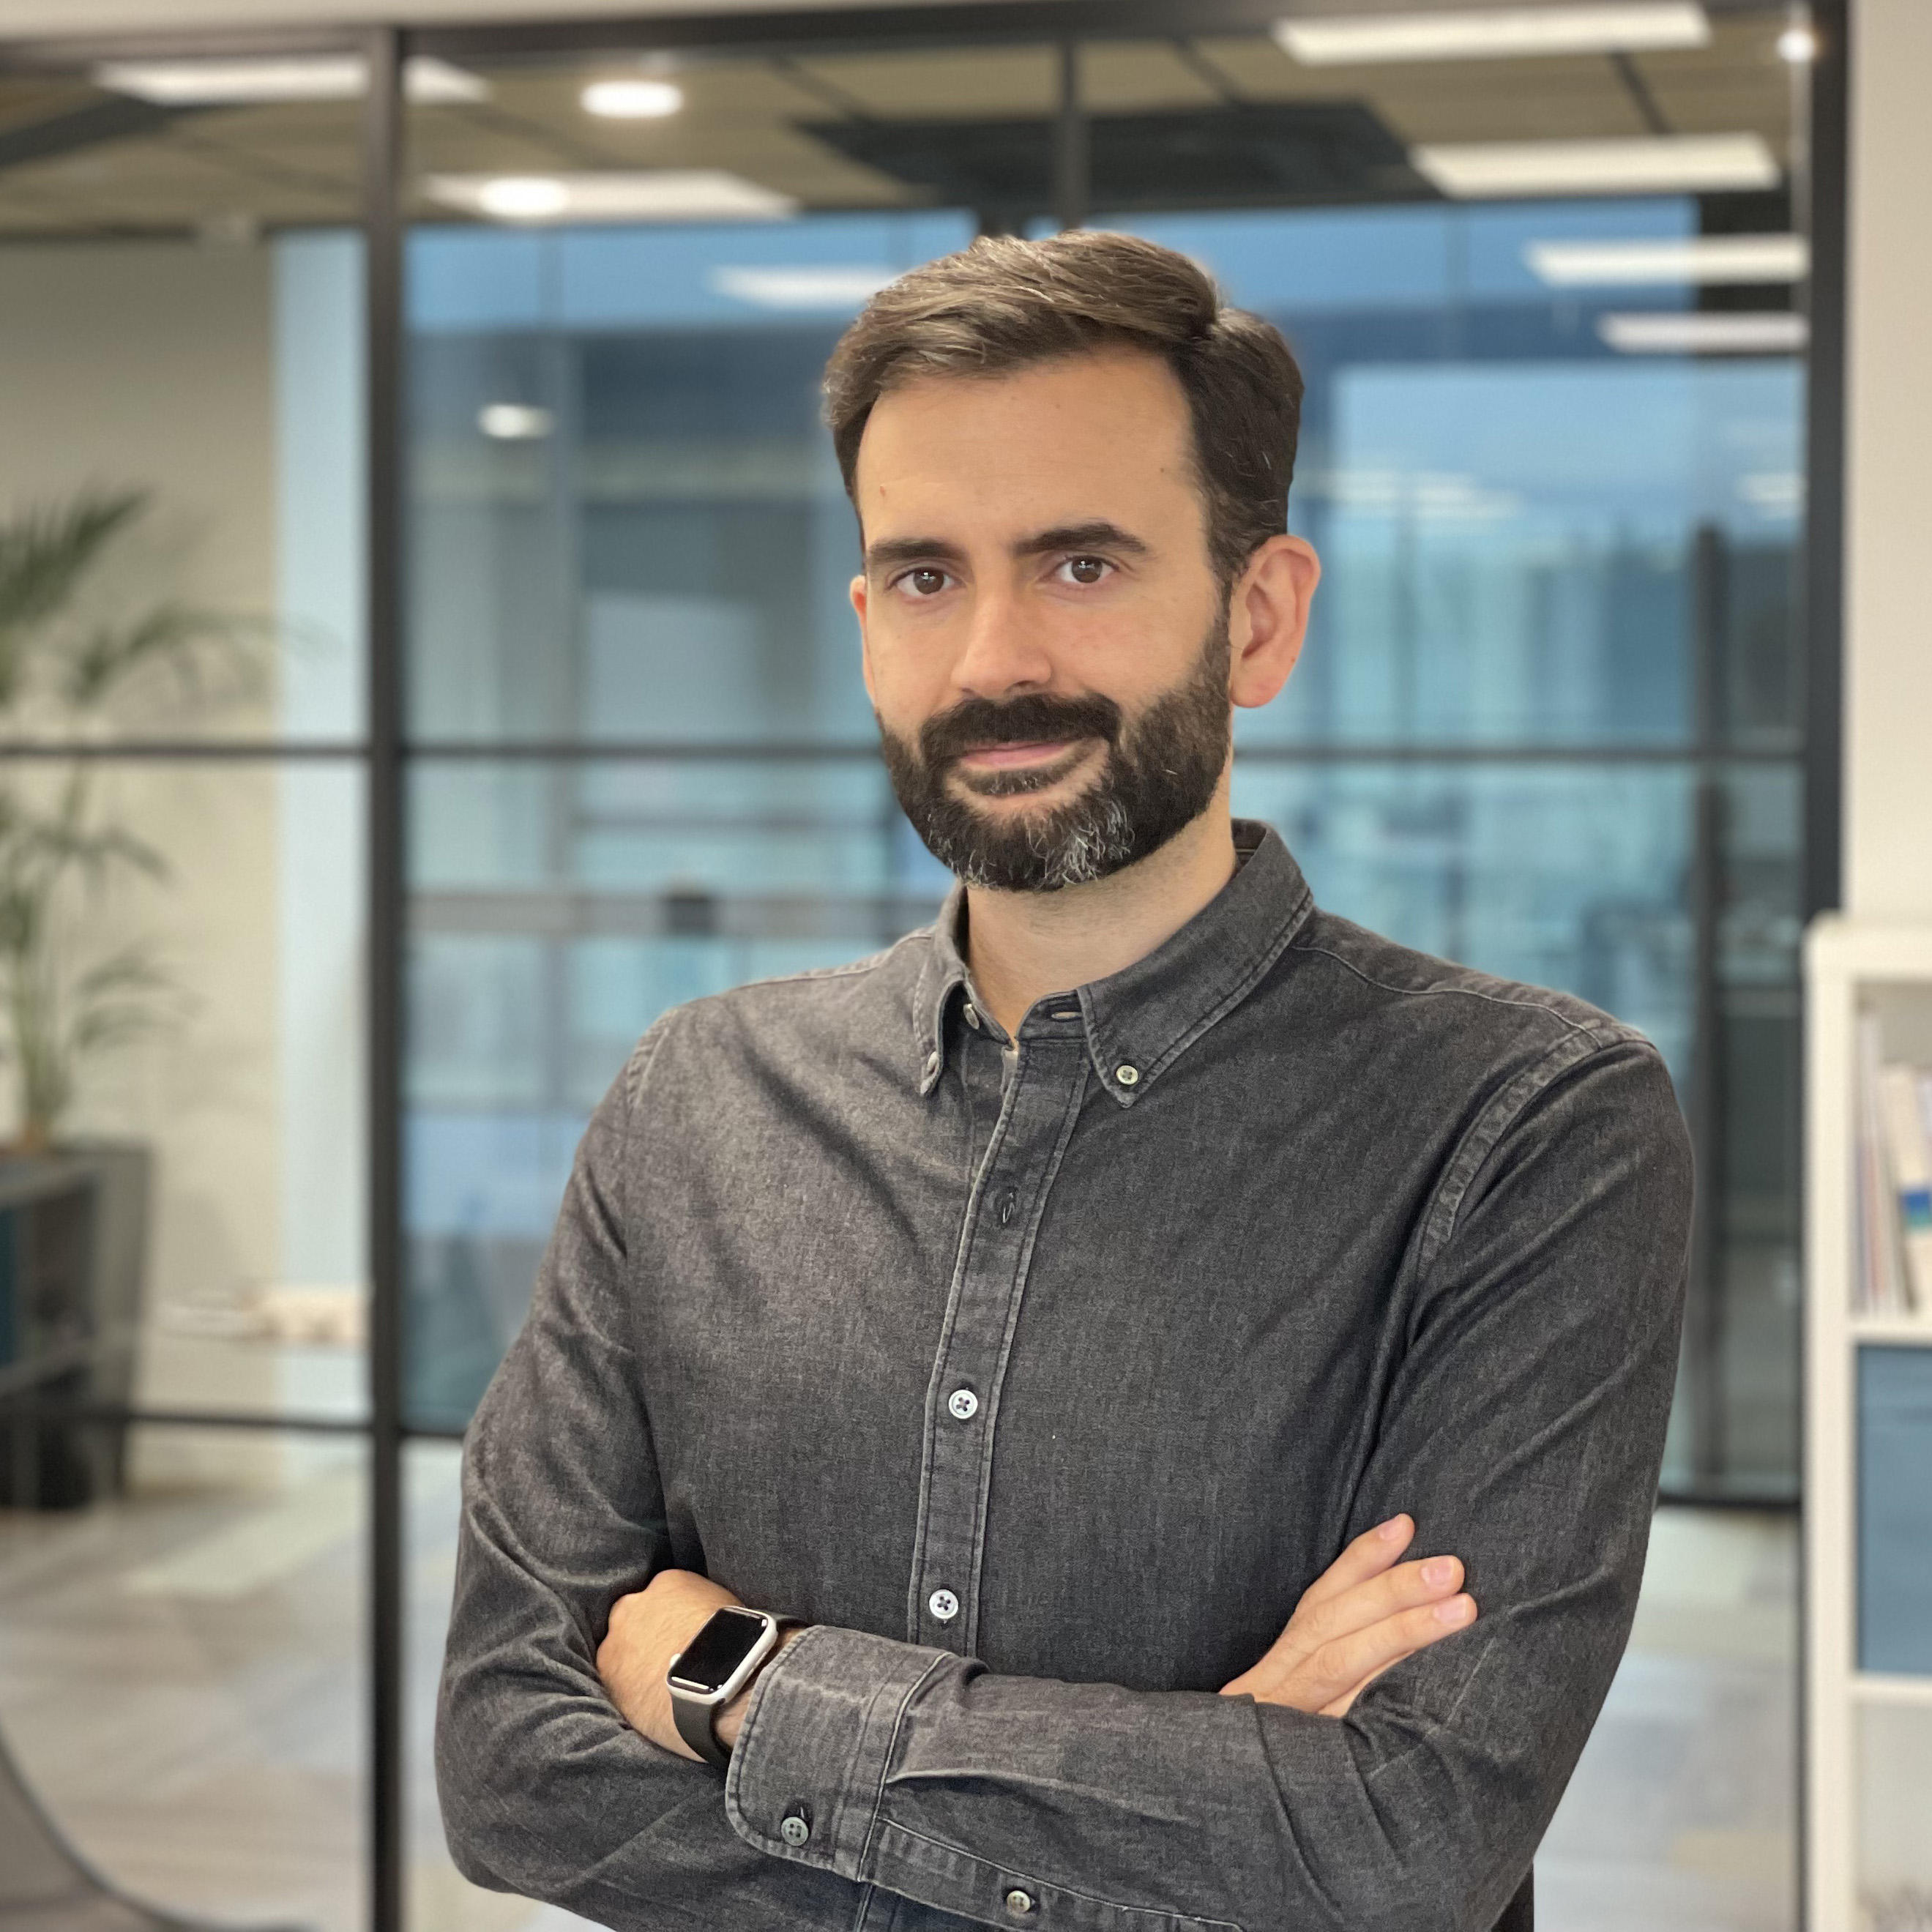
\includegraphics[width=1in,height=1.25in,clip,keepaspectratio]{illustrations/photo_rafa.jpg}
\end{wrapfigure}\par
\noindent \textbf{Rafael Pagés} is Co-Founder and CEO of Volograms, a startup bringing 3D reconstruction technologies to everyone. He received the Telecommunications Engineering degree (Integrated B.Sc.-M.Sc. accredited by ABET) in 2010, and PhD in Communication Technologies and Systems degree in 2016, both from Technical University of Madrid (UPM), in Spain. Rafael was member of the Image Processing Group at UPM and did his post-doctoral research at Trinity College Dublin. His research interests include 3D reconstruction, volumetric video, and computer vision.\\

\newpage %bring to right text column
\setlength\intextsep{0pt} % to bring image and text on same
\begin{wrapfigure}{l}{25mm} 
    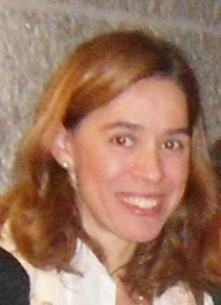
\includegraphics[width=1in,height=1.25in,clip,keepaspectratio]{illustrations/photo_clara.jpg}
\end{wrapfigure}\par
\noindent \textbf{Clara Pérez-Molina} received her M.Sc. degree in Physics from the Complutense University in Madrid and her PhD in Industrial Engineering from the Spanish University for Distance Education (UNED). She has worked as researcher in several National and European Projects and has published different technical reports and research articles for International Journals and Conferences, as well as several teaching books. She is currently an Associate Professor with tenure of the Electrical and Computer Engineering Department at UNED.
Her research activities are centered on Educational Competences and Technology Enhanced Learning applied to Higher Education in addition to Renewable Energy Management and Artificial Intelligence techniques. She is senior member of the IEEE.\\

\setlength\intextsep{0pt} % to bring image and text on same level
\begin{wrapfigure}{l}{25mm} 
    
\includegraphics[width=1in,height=1.25in,clip,keepaspectratio]{illustrations/photo_sergio_martin.png}
\end{wrapfigure}\par
\noindent \textbf{Sergio Martín} is Associate Professor at UNED (National University for Distance Education, Spain). He is PhD by the Electrical and Computer Engineering Department of the Industrial Engineering School of UNED. He is Computer Engineer in Distributed Applications and Systems by the Carlos III University of Madrid. He teaches subjects related to microelectronics and digital electronics since 2007 in the Industrial Engineering School of UNED. He has participated since 2002 in national and international research projects related to mobile devices, ambient intelligence, and location-based technologies as well as in projects related to "e-learning", virtual and remote labs, and new technologies applied to distance education. He has published more than 200 papers both in international journals and conferences. He is IEEE senior member.\\

